%File: formatting-instruction.tex
\documentclass[letterpaper]{article}

\usepackage{aaai}
\usepackage{courier}
\usepackage{graphicx}
\usepackage{helvet}
\usepackage{times}

\graphicspath{ {./images/} }

\frenchspacing
\setlength{\pdfpagewidth}{8.5in}
\setlength{\pdfpageheight}{11in}
\pdfinfo{
/Title (Using Automated Planning in data centers fault tolerance systems)
/Author (Douglas Trajano)}
\setcounter{secnumdepth}{2}  
 \begin{document}
% The file aaai.sty is the style file for AAAI Press 
% proceedings, working notes, and technical reports.
%
\title{Using Automated Planning in data centers fault tolerance systems}
\author{Douglas Trajano\\
Master's Degree in Computer Science\\
Pontifical Catholic University of Rio Grande do Sul - PUCRS\\
School of Technology. Porto Alegre, Brazil\\
douglas.trajano@edu.pucrs.br
}
\maketitle
\begin{abstract}
\begin{quote}
Data centers are key components for several companies and the digital transformation increases the quantity and the complexity of these IT assets. Develop intelligent systems that can be used in hardware failures is an area of study of artificial intelligence. With it in mind, we propose an automated planner to act or guide engineers in critical incidents to keep data centers healthy.
\end{quote}
\end{abstract}

\section{Introduction}

Nowadays, IT operations are crucial for business continuity. Information systems are used by companies in different processes and products, all these services are implemented in data centers. Critical incidents in data centers may impact the usability of these services and it needs to be handled in timely fashion by engineering team to avoid financial losses or affect their end users.

A data center is a building composed by computers systems, storage systems, infrastructure for power supply, telecommunications, environmental controls (e.g., air conditioning, fire suppression), and many others associated components. The complexity of these resources lies in the fact that all these components needs to work together, if one of these components have an issue, it can affects others components. Engineering teams needs to have a good knowledge of these components and their specific characteristics to be able to solve incidents. Knowledge bases for known issues are built in order to help engineers to apply solutions correctly and as soon as possible.

In this work we propose an automated planner that can understand known issues and provide a set of ordered actions to be implemented in the architecture to fix issues or apply workarounds solutions. We use Planning Domain Definition Language (PDDL) to modelling this domain and some problems (known issues). For each problem we can have different goals depends of the criticality of the situation. Nonetheless, our automated planner will provide a plan with the actions that are expected to achieve the goal.

This work is organized as follows. Section \ref{sec:approach} explain our approach in this work. Section \ref{sec:implementation} provides a detailed description of the proposed solution. Section \ref{sec:experiments} explains the experimental process and the results in detail. Section \ref{sec:related-work} discusses related works. Finally, section \ref{sec:conclusions} presents our conclusions and possibilities for future work.

\section{Approach}\label{sec:approach}
% What your idea is, and how it works
% Make sure your explanation will be clear to someone who's not already familiar with what you're doing

AI Planning is a field of Artificial Intelligence which explores the process of using autonomous techniques to solve planning and scheduling problems. A planning problem is one in which we have some initial starting state, which we wish to transform into a desired goal state through the application of a set of actions.

PDDL (Planning Domain Definition Language) is intended to express the "physics" of a domain, that is, what predicates there are, what actions are possible, what the structure of compound actions is, and what the effects of actions are.\cite{ghallab1998pddl}

We use PDDL to modeling our domain and some sample problems (known issues). The domain contains some components like worker computers, master computers, switches, storage devices, etc. interpreted as objects. The relationship between the components and their states are defined as predicate properties (properties which are either true or false). All possible actions that our planner can apply are defined as well in the domain file. Each problem definition contains the instances of our objects, the initial states and the goals for that problem. 

\section{Implementation}\label{sec:implementation}
% What it does, what language or system it's written in, etc.
% Use figures or screen dumps if appropriate

The domain and the problems are defined using PDDL. The automated planner and validator used in this project are provided by planning.domains: http://solver.planning.domains/

As explained early, data centers are complex systems with several hardware components, to validate our proposed solution, we focused in modeling the main components and their integration.

Our domain is composed of components of three types.

\subsection{Computer components}\label{sec:implementation1}

The computer resources defined in our domain are worker and master nodes.

Worker computers are used to deploy applications and are controlled by master computers through switches. Some predicates related with this resource are:

\begin{itemize}
    \item \textbf{worker-healthy}: Indicates if the worker is healthy or not.
    \item \textbf{worker-high-mem}: Indicates a high usage of memory.
    \item \textbf{worker-high-cpu}: Indicates a high usage of processor.
    \item \textbf{worker-high-network}: Indicates a high usage of network.
\end{itemize}

Master computers provides management tools for an entire cluster. All worker nodes attached in a switch will use these tools. 

\begin{itemize}
    \item \textbf{master-healthy}: Indicates if the master is healthy or not.
\end{itemize}

\subsection{Network components}\label{sec:implementation2}

Routers and switches are networks devices used in our implementation. All others components are connected by switches and exposes for the external world using the routers.

Routers expose clusters to the outside world, they work in pairs.

\begin{itemize}
    \item \textbf{router-healthy}: Indicates if the router is healthy or not.
    \item \textbf{router-pair}: Defines an integration between two routers.
\end{itemize}

Switches connect all components of the cluster and is attached in a router.

\begin{itemize}
    \item \textbf{switch-healthy}: Indicates if the switch is healthy or not.
    \item \textbf{switch-attach-router}: Establish a connection between a switch and a router.
    \item \textbf{switch-attach-master}: Establish a connection between a switch and a master computer.
    \item \textbf{switch-attach-worker}: Establish a connection between a switch and a worker computer.
\end{itemize}

\subsection{Storage components}\label{sec:implementation3}

We have two types of storage devices.

EBS is a block storage used by computers for their operating systems. Each EBS can be used by only one computer.

\begin{itemize}
    \item \textbf{ebs-healthy}: Indicates if the EBS is healthy or not.
    \item \textbf{ebs-locked}: Indicates if the EBS is locked or not.
    \item \textbf{ebs-attached}: Establish a connection between an EBS and a computer.
\end{itemize}

Bucket is a object storage attached in a master computer and shared with applications deployed in that cluster.

\begin{itemize}
    \item \textbf{bucket-healthy}: Indicates if the bucket is healthy or not.
    \item \textbf{bucket-locked}: Indicates if the bucket is locked or not.
    \item \textbf{bucket-attached}: Establish a connection between a bucket and a master computer.
\end{itemize}

The diagram below demonstrates how these components works together in a healthy scenario.

Each cluster receives the name of a famous scientist as a tribute. This has no practical effect on our architecture.

\begin{figure}[ht]
    \centering
    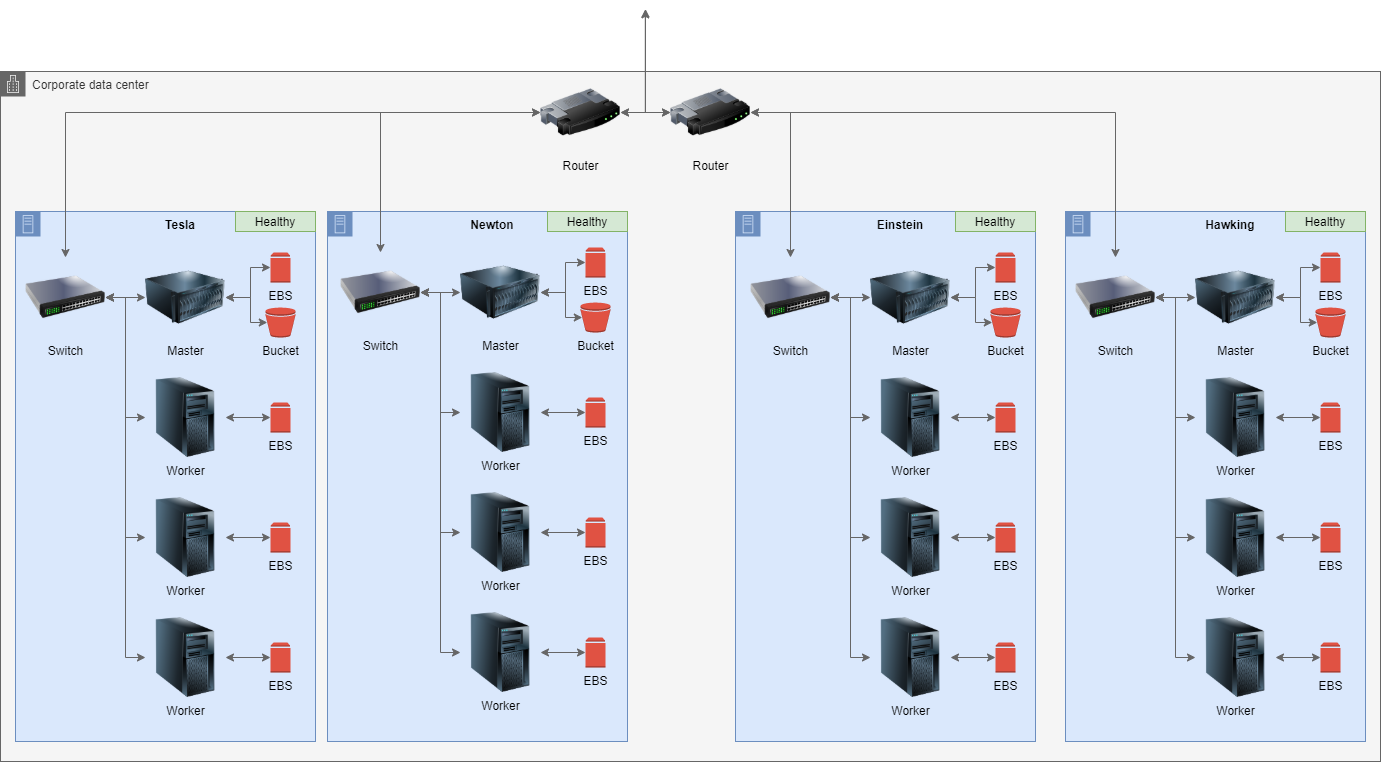
\includegraphics[width=8cm]{images/diagrams-healthy.png}
    \caption{Data Center Domain}
    \label{fig:data-center-domain}
\end{figure}

\section{Experiments}\label{sec:experiments}
% Purpose (e.g., experimental hypotheses you wanted to test)
% Experimental design
% Experimental results – Use tables or graphs (preferably graphs)
% What the results mean 

We want to validate that PDDL has flexibility to modeling different architectures of data centers, with more or less components, and different known issues that our engineers can define and maintain it using a common language. So, engineering teams can act more quickly on incidents using the planner as guide or allowing that the planner can apply the actions directly in the architecture.

Three different scenarios are explored in this work. As PDDL uses the domain and problem as definition, we will reference these scenarios as problems.

The goal of our three problems are the same, all components healthy and connected properly and no error message.

\subsection{Problem 1}\label{sec:experiments1}

The first problem explore an initial state of our data center. All components are turned off and needs to be turned on in a specific order. Firstly, routers and switches needs to be turned on, their are responsible to communicate with others objects. Worker and master nodes requires that storage devices are turned on previously.

\begin{figure}[ht]
    \centering
    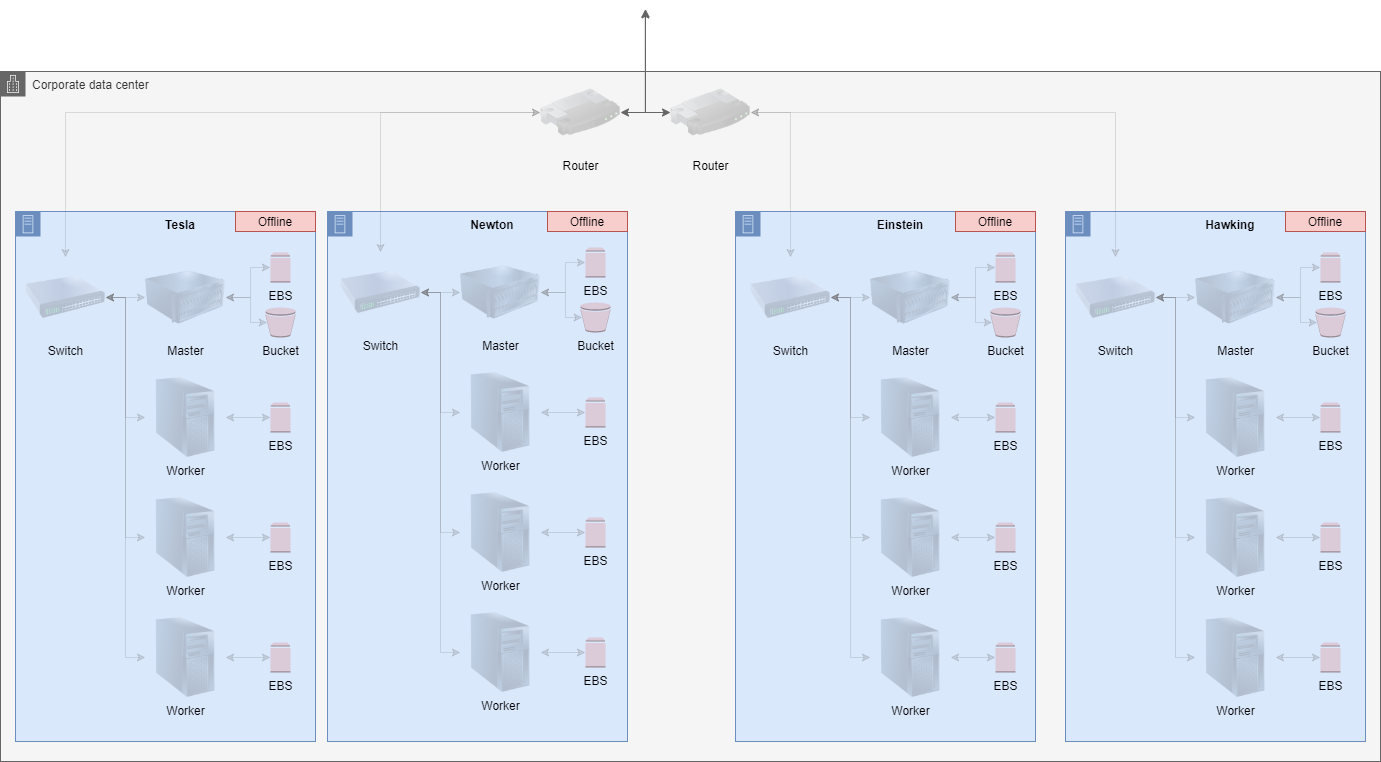
\includegraphics[width=8cm]{images/diagrams-pb1.png}
    \caption{Problem 1}
    \label{fig:data-center-pb1}
\end{figure}

The plan for this problem is shown below. Note that the solver respect the dependencies between the components, starting routers and switches firstly and the storage and computers in the sequence.

\textbf{router-turn-on} router1 

\textbf{switch-turn-on} switch1 router1 

\textbf{switch-turn-on} switch2 router1 

\textbf{switch-turn-on} switch3 router1 

\textbf{switch-turn-on} switch4 router1 

\textbf{router-turn-on} router2 

\textbf{router-mesh-on} router1 router2 

\textbf{ebs-turn-on} ebs1 

\textbf{worker-turn-on} w12 switch4 ebs1 

\textbf{ebs-turn-on} ebs2 

\textbf{worker-turn-on} w11 switch4 ebs2 

\textbf{ebs-turn-on} ebs3 

\textbf{worker-turn-on} w10 switch4 ebs3 

\textbf{ebs-turn-on} ebs4 

\textbf{worker-turn-on} w9 switch3 ebs4 

\textbf{ebs-turn-on} ebs5 

\textbf{worker-turn-on} w8 switch3 ebs5 

\textbf{ebs-turn-on} ebs6 

\textbf{worker-turn-on} w7 switch3 ebs6 

\textbf{ebs-turn-on} ebs7 

\textbf{worker-turn-on} w6 switch2 ebs7 

\textbf{ebs-turn-on} ebs8 

\textbf{worker-turn-on} w5 switch2 ebs8 

\textbf{ebs-turn-on} ebs9 

\textbf{worker-turn-on} w4 switch2 ebs9 

\textbf{ebs-turn-on} ebs10 

\textbf{worker-turn-on} w3 switch1 ebs10 

\textbf{ebs-turn-on} ebs11 

\textbf{worker-turn-on} w2 switch1 ebs11 

\textbf{ebs-turn-on} ebs12 

\textbf{worker-turn-on} w1 switch1 ebs12 

\textbf{ebs-turn-on} ebs13 

\textbf{ebs-turn-on} ebs14 

\textbf{ebs-turn-on} ebs15 

\textbf{ebs-turn-on} ebs16 

\textbf{bucket-turn-on} bucket1 

\textbf{master-turn-on} hawking switch4 ebs13 bucket1 

\textbf{bucket-turn-on} bucket2 

\textbf{master-turn-on} einstein switch3 ebs14 bucket2 

\textbf{bucket-turn-on} bucket3 

\textbf{master-turn-on} newton switch2 ebs15 bucket3 

\textbf{bucket-turn-on} bucket4 

\textbf{master-turn-on} tesla switch1 ebs16 bucket4

\subsection{Problem 2}\label{sec:experiments2}

In the second problem, we have some components in three different clusters with errors (memory, cpu and network). When the computer is restarted, its solved this issue.

\begin{figure}[ht]
    \centering
    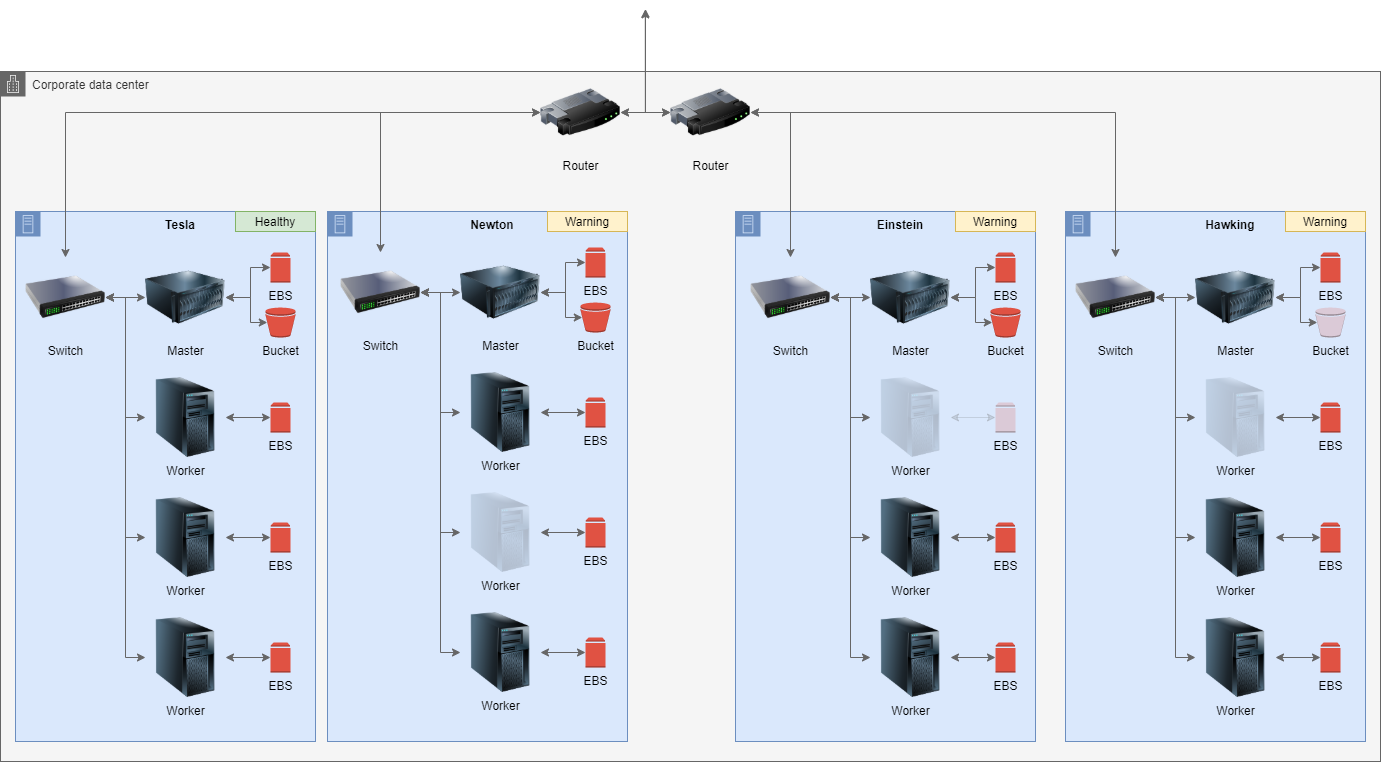
\includegraphics[width=8cm]{images/diagrams-pb2.png}
    \caption{Problem 2}
    \label{fig:data-center-pb2}
\end{figure}

Actually, some computers that are facing issues are healthy, but with error messages triggered. We defined only actions for turn on and turn off the components, so the solution found by the planner are turn off the problematic computers and turn on again. The plan for this problem is shown below.

\textbf{worker-turn-on} w7 switch3 ebs10 

\textbf{bucket-turn-on} bucket4 

\textbf{worker-turn-off} w5 switch2 ebs7 

\textbf{worker-turn-on} w5 switch2 ebs7 

\textbf{master-turn-off} hawking switch4 ebs13 bucket4 

\textbf{master-turn-on} hawking switch4 ebs13 bucket4 

\textbf{worker-turn-off} w10 switch4 ebs14 

\textbf{worker-turn-on} w10 switch4 ebs14

\subsection{Problem 3}\label{sec:experiments3}

In the third problem we have a cluster complete offline, all components needs to be turned on.

\begin{figure}[ht]
    \centering
    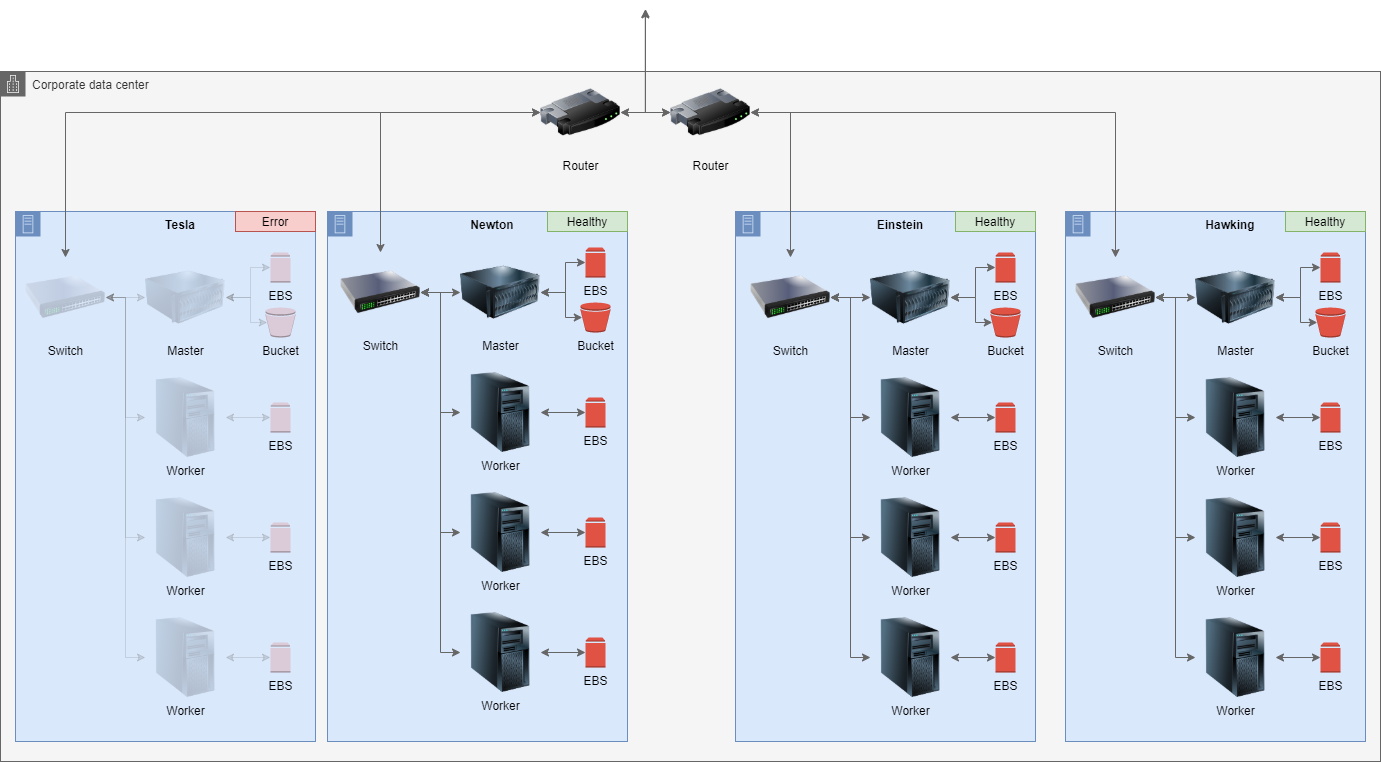
\includegraphics[width=8cm]{images/diagrams-pb3.png}
    \caption{Problem 3}
    \label{fig:data-center-pb3}
\end{figure}

The planner provided a sequence to turn on all the components related to tesla cluster. The plan for this problem is shown below.

\textbf{switch-turn-on} switch1 router1

\textbf{ebs-turn-on} ebs1

\textbf{worker-turn-on} w3 switch1 ebs1

\textbf{ebs-turn-on} ebs2

\textbf{worker-turn-on} w2 switch1 ebs2

\textbf{ebs-turn-on} ebs3

\textbf{worker-turn-on} w1 switch1 ebs3

\textbf{ebs-turn-on} ebs4

\textbf{bucket-turn-on} bucket1

\textbf{master-turn-on} tesla switch1 ebs4 bucket1


\section{Related work}\label{sec:related-work}
% What others have done
% Strengths and weaknesses of their work
% How it compares to your work

Few works addressed the usability of artificial intelligence systems in fault tolerance.

In "Predicting Remediations for Hardware Failures in Large-Scale Datacenters" \cite{lin2020predicting} a Gradient Boosted Decision Tree are trained using as input data server failure logs, tooling logs and server attributes for all solved incidents.

In "Predicting Computer System Failures Using Support Vector Machines" \cite{10.5555/1855886.1855891} the authors describes the usage Support Vector Machine (SVM) approach to predict failure events based on system log files.

These works are great and help to improve data center management. Our work is distinguished by provide a definition language that engineers can add new known issues very quickly to the system. Also, the explainability of the automated planner is a great benefit as it can be easily interpreted.

\section{Conclusions}\label{sec:conclusions}
%Summarize what you accomplished
% What significance or impact or meaning does it have?
% Honest assessment of the limitations of your work
%% What one could do overcome those limitations

%% Future work

The idea of using PDDL to formalize domains of data center architectures seems to be promising. Nonetheless, there are still many questions to be answered.

\begin{itemize}
    \item Is it reasonable to require PDDL skills for engineers? Their can develop and maintain the domain and problem files? 
    \item How the information represented by predicates will be collected for the planner?
    \item Can we allow the planner to act directly on the infrastructure? Should some actions be restricted to engineers?
\end{itemize}

As the future work, is interesting to explore more complex architectures, with more components, involving applications and more possible situations (problems). Define more appropriate actions for the components will provide better plans avoiding a sequence of turn off and turn on that can be stressful for the system. This work is just a small step towards a new possibility to manage infrastructure of our data centers.

\bibliographystyle{aaai}
\bibliography{references.bib}

\end{document}